%%%%%%%%%%%%%%%%%%%%%%%%%%%%%%%%%%%%%%%%%%%%%%%%%%%
%% P3: Phenomenology of Particle Physics                         
%%
%% Author:  André Rubbia                   		 
%%
%% Figure 2.13 Definition of the kinematical quantities relevant for the large-angle scattering experiment of Rutherford. 
%%
%% This work is licensed under the Creative Commons Attribution 4.0 International License. 
%% To view a copy of this license, visit http://creativecommons.org/licenses/by/4.0/ or 
%% send a letter to Creative Commons, PO Box 1866, Mountain View, CA 94042, USA.
%%
%%%%%%%%%%%%%%%%%%%%%%%%%%%%%%%%%%%%%%%%%%%%%%%%%%%

\documentclass[a4paper,10pt]{article}

\usepackage[T1]{fontenc}
\usepackage[utf8]{inputenc}
\usepackage{lmodern}
\usepackage[labelfont=bf]{caption}
\usepackage{upgreek}
\usepackage{amssymb}
\usepackage{amsmath}

\usepackage{tikz}
\usepackage{pgfplots}
\pgfplotsset{compat=1.17}
\usepgfplotslibrary{ternary}
\usepgfplotslibrary{fillbetween}
\usepgfplotslibrary{external}


\def\d{\mathrm{d}}

\begin{document}

%%%%%%%%%%%%%%%   FIGURE  %%%%%%%%%%%%%%%%%%%%%%%%%%%%%%
\begin{figure}[htb]
\begin{center}
%%%\includegraphics[width=0.55\textwidth]{BasicConcepts/streuexperiment.pdf}
    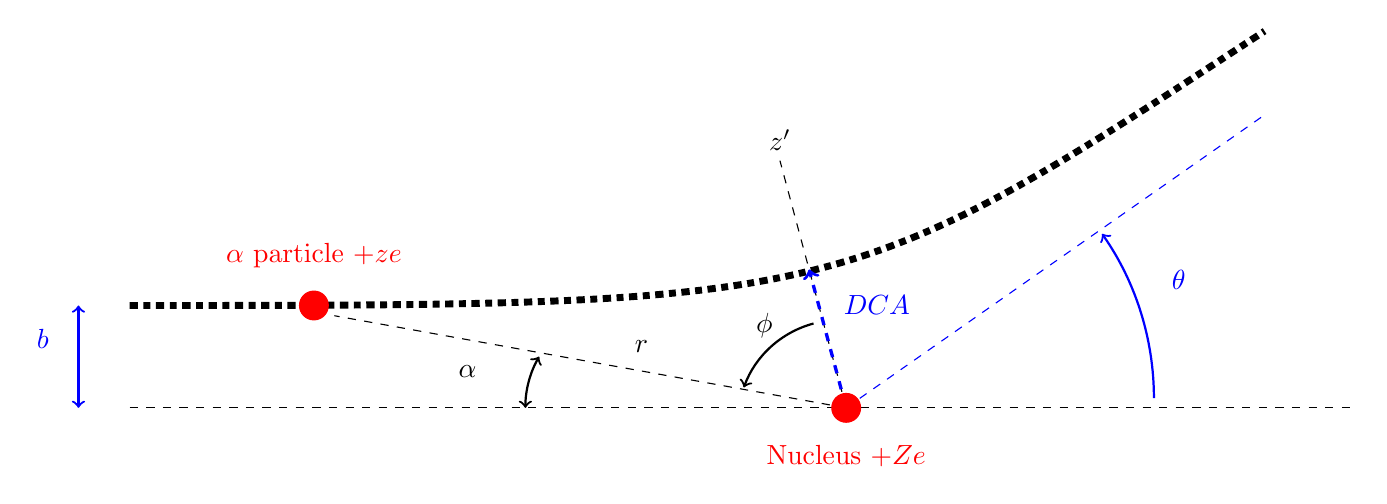
\begin{tikzpicture}[scale=1.3]

         \draw[dashed] (-7,0) -- (5,0);
         \draw[dashed] (0,0) -- (-5,0.9);
         \draw[dashed, blue] (0,0) -- (35:5);
         \draw[line width=2.5, dash dot] (-7,1) .. controls (0,1) .. (42:5.5);
         \draw[dashed] (0,0) -- (105:2.5) node[above] {$z^\prime$};
         \draw[<->,blue, dashed, very thick] (0,0) -- (105:1.4);
         \filldraw [red] (0,0) circle (4pt) node[below=10pt] {Nucleus $+Ze$};
         \filldraw [red] (-5.2,1) circle (4pt) node[above=10pt] {$\alpha$ particle $+ze$};
         \draw[thick,blue,<->] (-7.5,0) -- (-7.5,1) node[left=7pt, yshift=-12pt] {$b$};
         \draw[thick,blue,<-] (2.5,1.7) arc (35:0:2.8);
         \node[blue] at (3.25,1.25) {$\theta$};
         \node[blue] at (0.3,1)  {$DCA$};
         \node at (-2.,0.6) {$r$};
         \node at (-3.7,0.35) {$\alpha$};
         \draw[thick,<->] (-3,0.5) arc (150:180:1);
         \draw[thick,<-] (-1,0.2) arc (160:105:1);
         \node at (-0.8,0.8) {$\phi$};
  \end{tikzpicture}
\caption{Definition of the kinematical quantities relevant for the large-angle scattering experiment of Rutherford. The picture depicts the large-angle deviation due to a single atom. The impact parameter is $b$ (before the collision) and the resulting scattering angle is $\theta$. The position of the $\alpha$ particle along its trajectory is given by $(r,\alpha)$. The distance of closest approach is defined by $DCA$ along an axis $z^\prime$.}
\end{center}
\end{figure}
%%%%%%%%%%%%%%%   END FIGURE  %%%%%%%%%%%%%%%%%%%%%%%%%%%%%%

\end{document}
